\documentclass[a4paper,ngerman,12pt]{scrartcl}

\usepackage[utf8]{inputenc}
%\usepackage[ansinew]{inputenc}

\usepackage[ngerman]{babel}

\usepackage{amsmath,amsthm,amssymb,stmaryrd,color,graphicx}
\usepackage{setspace}
\usepackage{bussproofs}
\usepackage{array}
\usepackage{comment}
\usepackage{wrapfig}

\usepackage{enumitem}

\usepackage{units}

\usepackage[protrusion=true,expansion=true]{microtype}

\usepackage{lmodern}

\usepackage{hyperref}
\usepackage{cleveref}

\newcommand{\RR}{\mathbb{R}}
\newcommand{\CC}{\mathbb{C}}
\newcommand{\ZZ}{\mathbb{Z}}
\newcommand{\NN}{\mathbb{N}}
\newcommand{\QQ}{\mathbb{Q}}

\setlength\parskip{\medskipamount}
\setlength\parindent{0pt}

\theoremstyle{definition}
\newtheorem{defn}{Definition}[]
\newtheorem{axiom}[defn]{Axiom}
\newtheorem{bsp}[defn]{Beispiel}

\theoremstyle{plain}
\newtheorem{prop}[defn]{Proposition}
\newtheorem{motto}[defn]{Motto}
\newtheorem{wunder}[defn]{Wunder}
\newtheorem{ueberlegung}[defn]{Überlegung}
\newtheorem{lemma}[defn]{Lemma}
\newtheorem{kor}[defn]{Korollar}
\newtheorem{hilfsaussage}[defn]{Hilfsaussage}
\newtheorem{satz}[defn]{Satz}
\newtheorem{frage}[defn]{Frage}

\theoremstyle{remark}
\newtheorem{bem}[defn]{Bemerkung}
\newtheorem{aufg}[defn]{Aufgabe}

\newtheorem*{antwort}{Antwort}

\newlength{\aufgabenskip}
\setlength{\aufgabenskip}{1.4em}
\newcounter{aufgabennummer}
\newenvironment{aufgabe}[1]{
	\addtocounter{aufgabennummer}{1}
	\textbf{Aufgabe \theaufgabennummer.} \emph{#1} \par
}{\vspace{\aufgabenskip}}

\clubpenalty=10000
\widowpenalty=10000
\displaywidowpenalty=10000

\setlength\unitlength{1cm}

\usepackage{tikz}

\RequirePackage{geometry}
\geometry{textwidth=16.0cm,textheight=24.5cm,footskip=1.5cm}

\begin{document}
	
\begin{picture}(0,0)
\put(0,-0.5){%
	
\includegraphics[scale=0.1]{logo-ifm}
}
\put(14.0,-3.5){%
	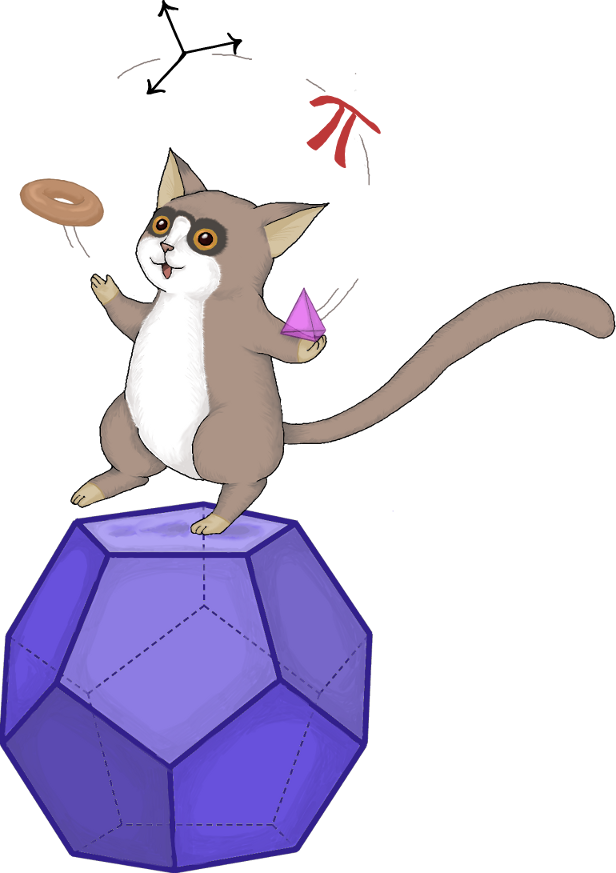
\includegraphics[scale=0.17]{cover}
}
\end{picture} 
	
\vspace{6em}

\begin{center}\Large{Siebter Korrespondenzbrief}\end{center}

\section*{Codierungstheorie}

Einleitung...

\section{Einführung}

Eine besonders einfache Methode Fehler bei der Übertragung zu erkennen, ist die Folgende: Man sendet die zu übertragende Nachricht einfach zweimal hintereinander. Passiert beim Übertragen der Nachricht ein Fehler, so erkennt der Empfänger das daran, dass die beiden Hälften der Nachricht nicht mehr gleich sind.

\begin{bsp}	
	Wollen wir bspw. das Wort \texttt{JUNI} übertragen, so senden wir stattdessen das Codewort \texttt{JUNIJUNI}. Passiert beim Übertragen ein einzelner Fehler (ein Buchstabe wird verfälscht), so erhält der Empfänger bspw. das Wort \texttt{JU\textbf{L}IJUNI} und kann direkt sehen, dass ein Fehler passiert sein muss.
\end{bsp}

Wir können es also erkennen, wenn bei der Übertragung ein Fehler passiert - wir können diesen Fehler aber nicht korrigieren (denn wir wissen ja nicht welche der beiden Hälften des Codewortes die korrekte ist). Außerdem können wir nur dann sicher sein, Fehler zu erkennen, wenn höchstens ein Fehler passiert. Treten bei der Übertragung zwei oder mehr Fehler auf, so kann es passieren, dass der Empfänger das nicht mehr erkennen kann:
	\begin{center}
		\texttt{JUNIJUNI} $\xrightarrow{\hspace*{2cm}}$ \texttt{JU\textbf{L}IJU\textbf{L}I}
	\end{center}

\begin{aufgabe}{}\label{aufgabe:verdreifachungsCodierung}
	Kannst du das oben beschriebene Verfahren so anpassen, dass ein einzelner Fehler vom Empfänger nicht nur erkannt, sondern auch korrigiert werden kann?
	
	Kannst du das Verfahren so anpassen, dass er auch zwei Fehler noch in jedem Fall erkennen kann?
\end{aufgabe}

Diese einfachen Codierungsverfahren funktionieren zwar grundsätzlich, haben aber einen großen Nachteil. Die zu übertragenden Nachrichten werden erheblich größer als die eigentliche Nachricht. Ein zentrales Ziel der Codierungstheorie ist es daher möglichst effiziente Codierungsverfahren zu finden, die die Nachrichten also nur wenig größer machen, aber es trotzdem erlauben Fehler zu erkennen (und evtl. sogar zu korrigieren).

Bevor wir uns auf die Suche nach solchen Verfahren machen können, müssen wir erst noch genauer festlegen, wie wir die Effizienz eines Codierungsverfahrens bestimmen wollen. Dazu werden wir ab sofort nur noch Verfahren der folgenden Form betrachten: 
\begin{enumerate}
	\item Teile die zu übertragende Nachricht in Stücke gleicher Länge ein. Diese Stücke nennen wir \emph{Wörter}. 
	\item Ersetze jedes der Wörter durch ein ihm zugeordnetes \emph{Codewort} - diese Codewörter müssen dabei ebenfalls alle eine einheitliche Länge haben.
	\item Schreibe die Codewörter wieder hintereinander und erhalte so die zu übertragende Nachricht.
\end{enumerate}

\begin{bsp}\label{bsp:Verdopplungscodierung}
	Wollen wir zum Beispiel die Verdopplungscodierung von oben mit einer Wortlänge von $4$ anwenden, um die Nachricht \texttt{DIESISTEINETESTNACHRICHT} zu übertragen, so funktionieren die Schritte wie folgt:
	\begin{enumerate}
		\item Teile die Nachricht in Wörter der Länge $4$: \texttt{DIES ISTE INET ESTN ACHR ICHT}
		\item Ersetze die Wörter durch ihre Codewörter: \texttt{DIES} $\rightarrow$ \texttt{DIESDIES}, \texttt{ISTE} $\rightarrow$ \texttt{ISTEISTE}, \dots
		\item Erhalte die codierte Nachricht: \texttt{DIESDIESISTEISTEINETINETESTNESTNACHRNACHRICHTICHT}
	\end{enumerate}
\end{bsp}

\begin{aufgabe}{}
	Selber ausprobieren?
\end{aufgabe}

Für Verfahren der oben beschriebenen Form, können wir nun ganz einfach bestimmen, wie effizient sie sind:

\begin{defn}
	Als \emph{Informationsrate} eines bestimmten Codierungsverfahrens bezeichnet man das Verhältnis aus der Länge der Codewörter zur Länge der Nachrichtenwörter, also die Zahl
		\[\frac{\text{Länge eines Codewortes}}{\text{Länge eines Nachrichtenwortes}}\]
	Je kleiner diese Zahl ist, desto effizienter ist das Verfahren.
\end{defn}

\begin{bsp}
	Für das Verdopplungscodierungsverfahren aus \Cref*{bsp:Verdopplungscodierung} ist die Informationsrate also:
		\[\frac{\text{Länge eines Codewortes}}{\text{Länge eines Nachrichtenwortes}} = \frac{4}{8} = 2\]
	Eine mit diesem Verfahren codierte Nachricht benötigt also doppelt so viel Platz wie die ursprüngliche Nachricht.
\end{bsp}

\begin{aufgabe}{}\label{aufgabe:verdreifachungsCodierungIR}
	Bestimme die Informationsrate für deine in Aufgabe 1 gefundenen Verfahren.
\end{aufgabe}

Als weitere Vereinfachung werden wir im restlichen Brief nur noch Nachrichten (und Codierungen) betrachten, die ausschließlich aus Zahlen bestehen. Das ist aber keine wirkliche Einschränkung, denn wie du schon im Kryptographie-Brief gesehen hast, lassen sich Buchstaben auch leicht durch Zahlen darstellen.


\section{Fehlererkennung}

Als erstes wollen wir uns nun mit Verfahren beschäftigen, die es uns erlauben einzelne Fehler zu erkennen. Das Verfahren soll dabei die folgende Form haben: Wir nehmen das Wort aus der Nachricht und codieren es, indem wir noch \glqq irgendetwas\grqq{} daran anhängen. Dieses \glqq irgendetwas\grqq{} soll es dem Empfänger dann erlauben einen möglicherweise aufgetretenen Fehler zu erkennen.
	\begin{center}
		\texttt{1847} $\xrightarrow{\hspace*{2cm}}$ \texttt{1847\_\_\_}
	\end{center}

Im ersten Kapitel war dieses \glqq irgendetwas\grqq{} zum Beispiel einfach wieder das Wort selbst. Das ist aber ziemlich ineffizient, da das Wort dadurch gleich doppelt so lang wird. Besser wäre es da schon nur die Quersumme des Wortes (das ist die Summe der einzelnen Ziffern) anzuhängen. Sind die Wörter vier Ziffern lang, so kann die Quersumme höchstens $9+9+9+9=36$ sein - uns genügt also ein zweistelliges Anhängsel.

\begin{bsp}
	Wollen wir die Nachricht $1701$ übertragen, so bilden wir die Quersumme $1+7+0+1=9$ und erhalten damit das Codewort $1701\textbf{09}$. Passiert beim Übertragen nun ein Fehler, so erhält der Empfänger beispielsweise die Nachricht $\textbf{8}70109$. Dieser kann nun leicht erkennen, ob ein Fehler aufgetreten ist, indem er einfach wieder die Quersumme der ersten vier Ziffern bildet ($8+7+0+1=16$) und mit den letzten beiden Ziffern vergleicht. Stimmen diese beiden Zahlen nicht überein, so weiß der Empfänger, dass beim Übertragen ein Fehler passiert sein muss.
\end{bsp}

\begin{aufgabe}{}
	Du bist der Empfänger und erhältst die folgenden Codewörter (die ursprünglichen Wörter hatten die Länge $4$):
		\[172919 \quad-\quad 422416 \quad-\quad 939124  \quad-\quad 314109\]
	Prüfe für jedes der Wörter, ob beim Übertragen ein Fehler aufgetreten ist. Falls nein, gib das ursprüngliche (uncodierte) Wort an. Falls ja, gib zwei Möglichkeiten an, wie das ursprüngliche Wort gelautet haben könnte (unter der Annahme, dass bei der Übertragung höchstens eine Ziffer verändert wurde). 
	
	Bei folgendem Codewort, ist bei der Übertragung etwas spezielles passiert - kannst du erklären was?
		\[739150\]
\end{aufgabe}

Funktioniert dieses Verfahren auch? D.h. können wir damit wirklich jeden einzeln auftretenden Fehler erkennen? Ja, denn wann immer eine einzelne Ziffer verändert wird, so ändert sich auch die Quersumme der ganzen Zahl. 

Ist das Verfahren effizient? Nun, die Informationsrate ist $\frac{\text{Länge eines Codewortes}}{\text{Länge eines Nachrichtenwortes}} = \frac{6}{4} = 1,5$ - also auf jeden Fall schonmal besser als bei dem bisherigen Verfahren.

Tatsächlich geht es aber sogar noch besser: Denn wenn nur eine einzelne Ziffer in der Nachricht verfälscht wird, dann kann sich die Quersumme doch höchstens um $9$ verändern. Es genügt also völlig, wenn wir uns nur die Einerstelle der Quersumme merken (oder anders ausgedrückt: Den Rest der Quersumme bei Division durch $10$). 

\begin{bsp}
	Um mit diesem Verfahren die Nachricht $8245$ zu übertragen, bilden wir also erneut die Quersumme $8+2+4+5=19$ und nehmen deren Einerstelle $9$. So erhalten wir das Codewort $8245\textbf{9}$.
\end{bsp}

\begin{aufgabe}{}
	Du empfängst die folgenden Codewörter - bei welchen von ihnen muss ein Fehler bei der Übertragung passiert sein?
		\[23836 \quad-\quad 99999 \quad-\quad 47629 \quad-\quad 38425\]
\end{aufgabe}

\begin{aufgabe}{}
	Bestimme die Informationsrate dieses Codierungsverfahrens.

	\emph{Zusatzaufgabe:} Kannst du das Verfahren irgendwie so verändern, dass die Informationsrate noch niedriger wird?
\end{aufgabe}


Rest 10

Vertauschung

\begin{bsp}
	ISBN
\end{bsp}

\begin{aufgabe}{}
	Bestimme Informationsrate von ISBN
\end{aufgabe}

\begin{aufgabe}{}
	Prüfe, ob folgende ISBN-Nummern korrekt abgetippt wurden.
\end{aufgabe}

\begin{bsp}
	Geldscheine
\end{bsp}


\section{Fehlerkorrektur und Güteanalyse}

\begin{defn}
	Hamming-Abstand
\end{defn}

Zusammenhang zwischen Hamming-Abstand und Fehlererkennung und -korrektur.

\begin{bsp}
	ISBN und Parity-Check
\end{bsp}

2-dimensionaler Parity-Check

Hamming-Abstand-Bestimmen? (Zumindest für n=2)

\begin{aufgabe}{}
	Bestimme Informationsrate (vgl. mit \Cref{aufgabe:verdreifachungsCodierungIR})
\end{aufgabe}

\begin{aufgabe}{}
	Konkrete Beispiele für Codierung/Decodierung
\end{aufgabe}

Perfekte/MDS-Codes?

\end{document}